

\section{2. Principe de la visualisation 3D}



\begin{frame}[t]
\frametitle{2. Principe de la visualisation 3D}
\begin{block}{M�canisme comparable en 3D:}
\begin{itemize}
\item Classe semie abstraite: \class{Display3D}
\item M�me principe: op�rateur \texttt{< \hspace{-0.2cm}<} et concept \class{CDrawableWithDisplay3D}
\item Deux classes h�ritent de \class{Display3D}: \class{Viewer3D} et \class{Board3D2D}  
\end{itemize}
\end{block}
\only<1,2,3>{\visible<2-> { \begin{block}{Visualisation bas�e \textit{OpenGL}: \class{Viewer3D}}
\begin{itemize}
\item Utilisation de la biblioth�que \textit{LibQLViewer} \footnote{\url{http://www.libqglviewer.com}}
\item H�rite � la fois de \texttt{Display3D} et \texttt{QGLViewer}.
\item<3> [+] Visualisation 3D interactive (possibilit� de s�lectionner des objets 3D). 
\item<3> [+] Fonctionnement simple.
\item<3> [+] Toujours maintenue depuis 2005 (derni�re version Juin 2010). 
\item<3> [-] D�pendance avec \textit{QT}. 
\item<3> [-] Export vectoriel possible (th�oriquement mais limit�).
\end{itemize}\end{block}}}%
\only<4>{
\begin{block}{Visualisation bas�e \textit{CAIRO}:  \class{Board3DTo2D} (Martial Tola)}
\begin{itemize}
\item M�me principe mais pas d'interaction.
\item [+] Pas de d�pendance \textit{QT}/carte 3D. 
\item [+] Export qualit� vectoriel.
\item [-] Positionnement manuel de la cam�ra. 
\item [-] Potentiellement moins riche compar� � \textit{OpenGL}. 
\end{itemize}
\end{block}
}
\end{frame}



\begin{frame}
\frametitle{2. Principe de la visualisation 3D}

\begin{block}{Classes v�rifiant le concept \class{CDrawableWithDisplay3D} }
\begin{center}
\begin{tabular}{lcc}
Classe & 3DViewer & Board3DTo2D \\
\class{PointVector} & X & X \\
\class{DigitalSetBySTLSet} & X & X \\
\class{DigitalSetBySTLVector} & X & X \\
\class{Object} & X & X \\
\class{HyperRectDomain} & X & X \\
\class{KhalimskyCell} & X & bient�t \\
\class{SignedKhalimskyCell} & X & bient�t
\end{tabular}
\end{center}

\end{block}


\end{frame}





\begin{frame}
\frametitle{Exemple de visualisations 3D}
\only<1>{
\begin{block}{Visualisation bas�e \class{Viewer3D}}
\begin{center}
\begin{tabular}{cc}
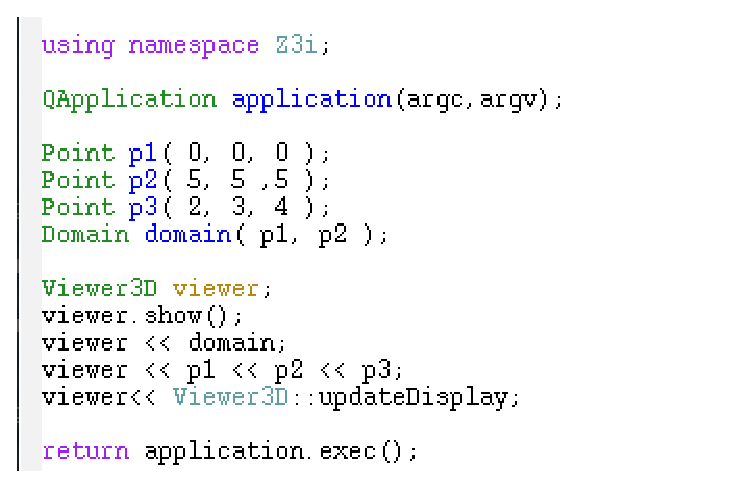
\includegraphics[height=0.33\textwidth]{Images/codeEx3DViewer.eps}&
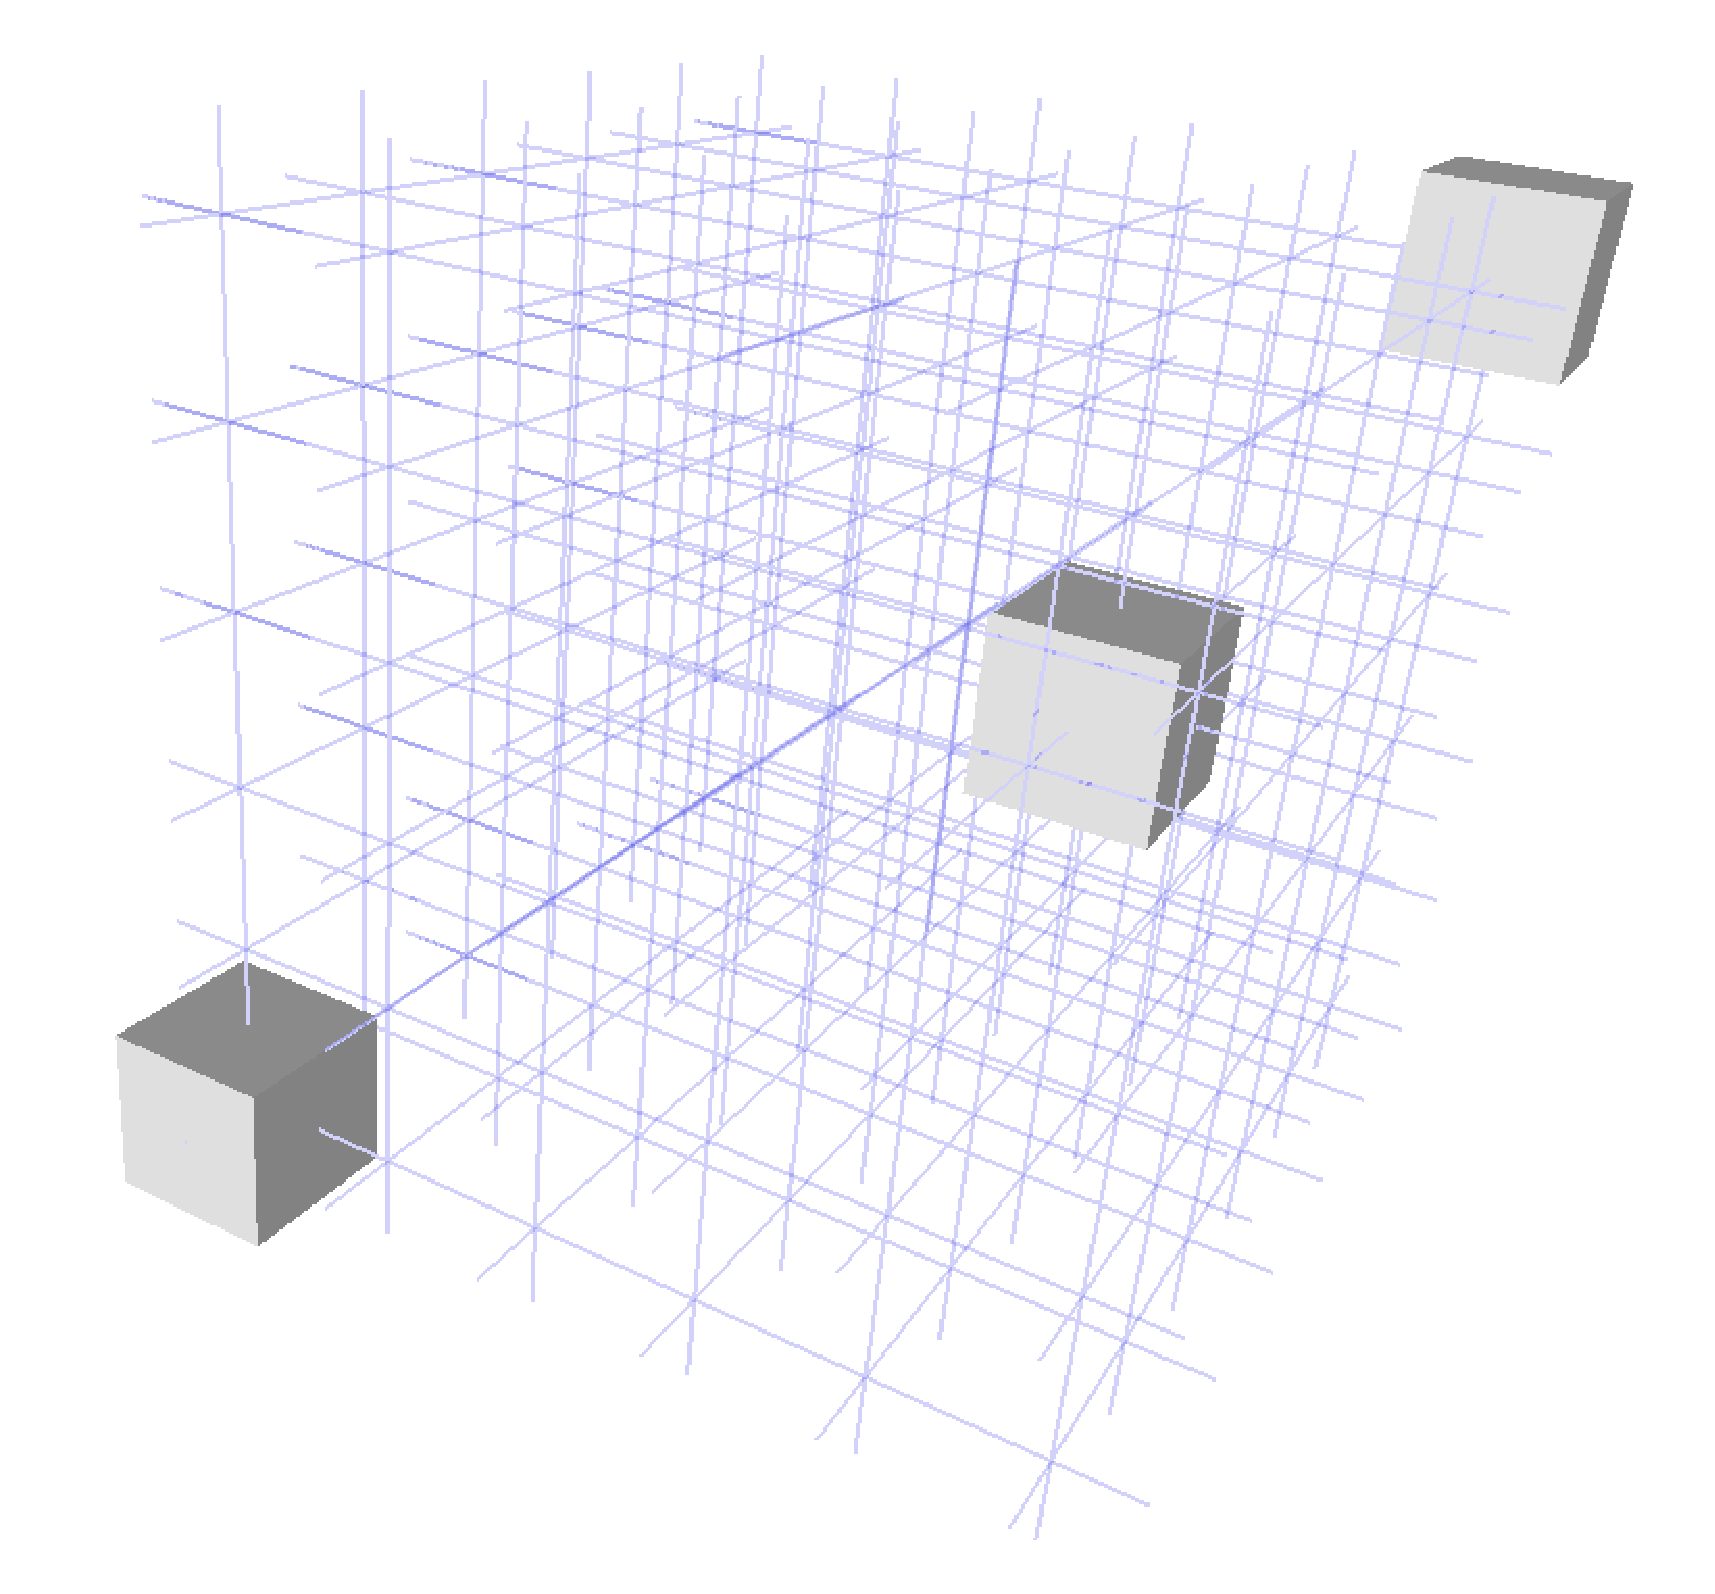
\includegraphics[height=0.33\textwidth]{Images/simple3dVisu1.eps}
\end{tabular}
\end{center}
\end{block}}

\only<2>{
\begin{block}{Visualisation bas�e \class{Board3DTo2D}}
\begin{center}
\begin{tabular}{cc}
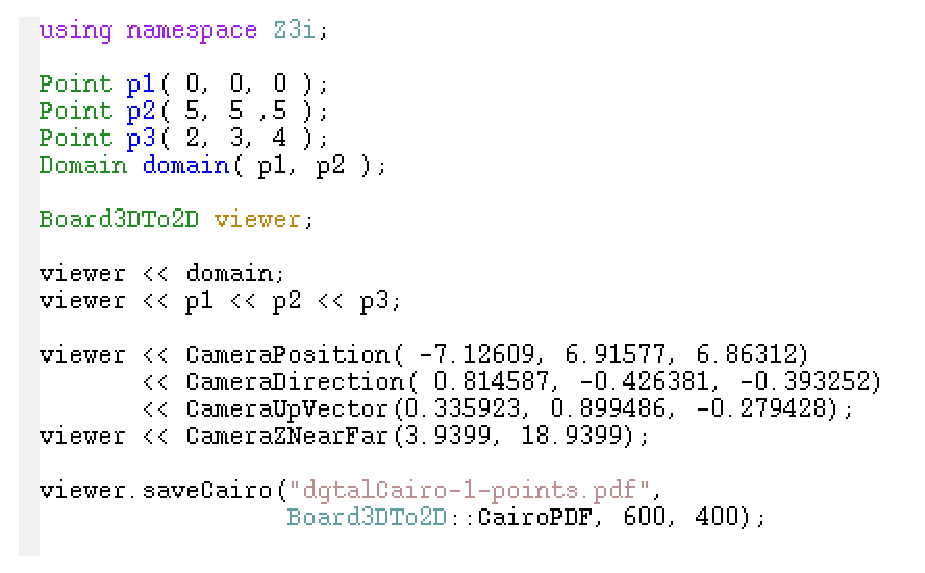
\includegraphics[height=0.33\textwidth]{Images/codeExBoard3D.eps}&
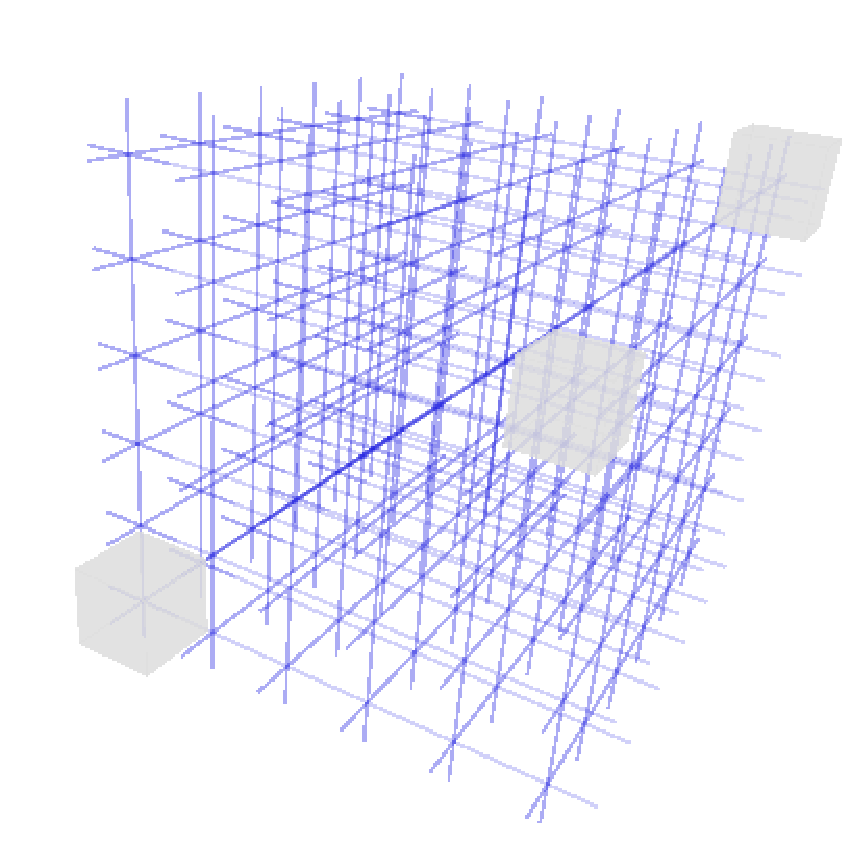
\includegraphics[height=0.33\textwidth]{Images/dgtalCairo-1-points.eps}
\end{tabular}
\end{center}
\end{block}
}

\end{frame}







\section{3. Modes de visualisation 3D}





\begin{frame}
\frametitle{3. Modes de visualisation 3D}

\begin{block}{Modification du style d'affichage}
D�finie pour chaque primitive:
\begin{semiverbatim}
viewer  \texttt{< \hspace{-0.2cm}<}  SetMode3D( p1.styleName(), "Grid" );
\end{semiverbatim}

\end{block}

\begin{block}{Diff�rents modes possibles: }
\begin{center}
\begin{tabular}{l|l}
Classe & modes \\ \hline

\class{PointVector} &  "Paving" (defaut), "Grid"\\
\class{DigitalSetBySTLSet} &  "Paving" (default), "PavingTransp", "Grid" \\
\class{DigitalSetBySTLVector}& "Paving" (default), "PavingTransp", "Grid" \\
\class{Object} &  "DrawAdjacencies", "PavingTransp" \\
\class{HyperRectDomain} & "Grid" (default), "Paving", "PavingPoints", \\
                        & "PavingGrids", "BoundingBox"\\
\class{KhalimskyCell} &  "Highlighted" ,"Transparent", "Basic"\\
\class{SignedKhalimskyCell} &  "Highlighted" ,"Transparent", "Basic".\\
\end{tabular}
\end{center}

\end{block}


\end{frame}








\begin{frame}[t]
\frametitle{3. Modes de visualisation 3D}

\begin{center}
\begin{tabular}{cccc}
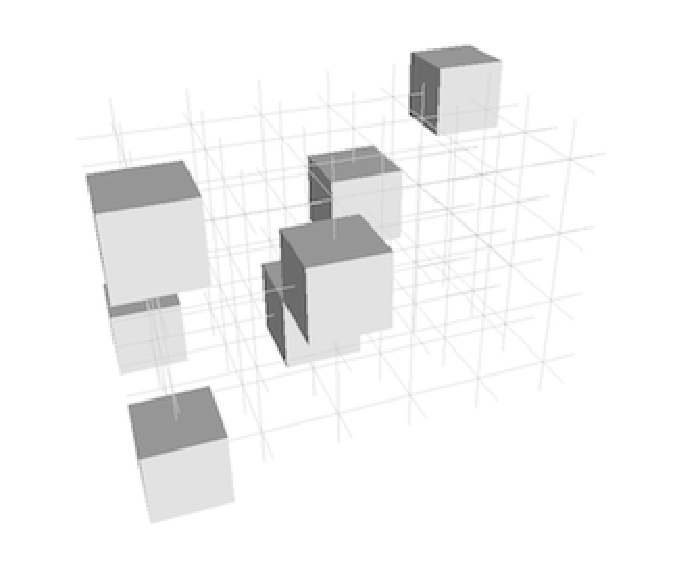
\includegraphics[width=0.3\textwidth]{Images/visuModeDefault.eps}&
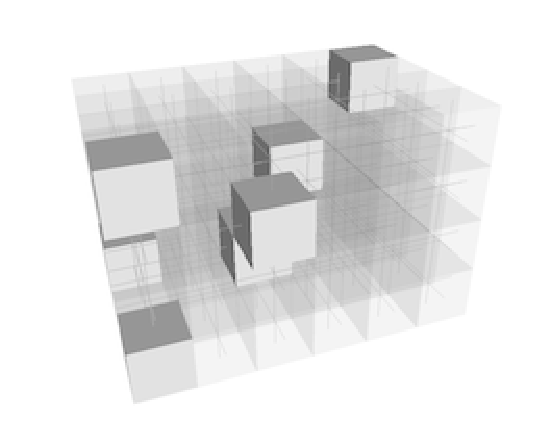
\includegraphics[width=0.3\textwidth]{Images/visuModePavingGridsDomain.eps}&

\includegraphics[width=0.3\textwidth]{Images/visuModeGridVoxel.eps}\\
mode  "" (Default) &  mode ``PavingGrids'' & mode ``Grid''
\end{tabular}
\end{center}

\end{frame}






\begin{frame}[t]

\frametitle{3. Modes de visualisation 3D }

\begin{block}{Visualisation personnalis�e}
\begin{semiverbatim}
viewer  \texttt{< \hspace{-0.2cm}<} CustomColors3D(Color(250, 0,0),Color(250, 0,0));
\end{semiverbatim}

\begin{center}
\includegraphics[width=0.6\textwidth]{Images/visuModeCustom-1.eps}
\end{center}
\end{block}
\end{frame}




\begin{frame}[t]
\frametitle{Exemples sur d'autres primitives }

\begin{center}
\begin{tabular}{c@{}c@{}c}
\includegraphics[height=0.22\textwidth]{Images/autrePrimitive3.eps}&
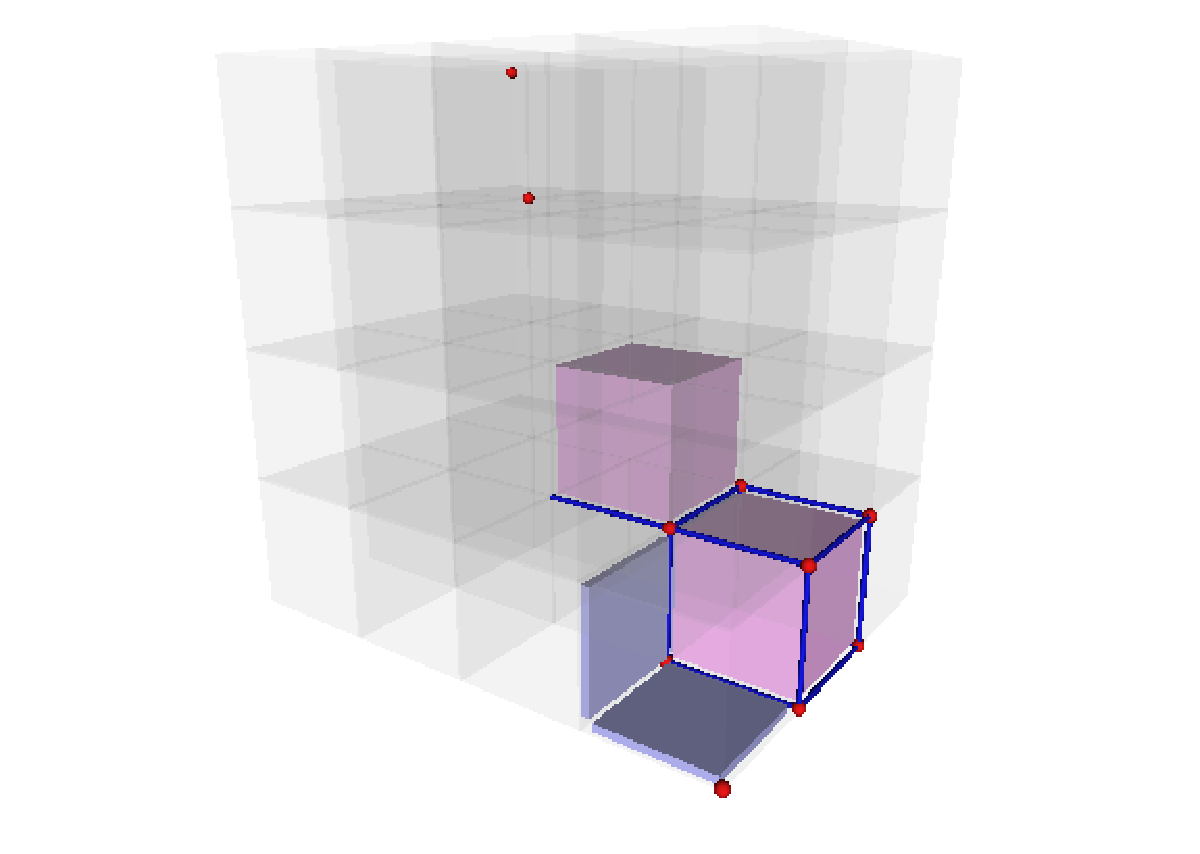
\includegraphics[height=0.22\textwidth]{Images/autrePrimitive2.eps}&
\includegraphics[height=0.22\textwidth]{Images/autrePrimitive.eps}\\
{\scriptsize{\class{Object} mode ``DrawAdjacencies''}} &{\scriptsize{\class{Khalimsky} Cells }}  & 
{\scriptsize{Signed \class{Khalimsky} Cells }} \\
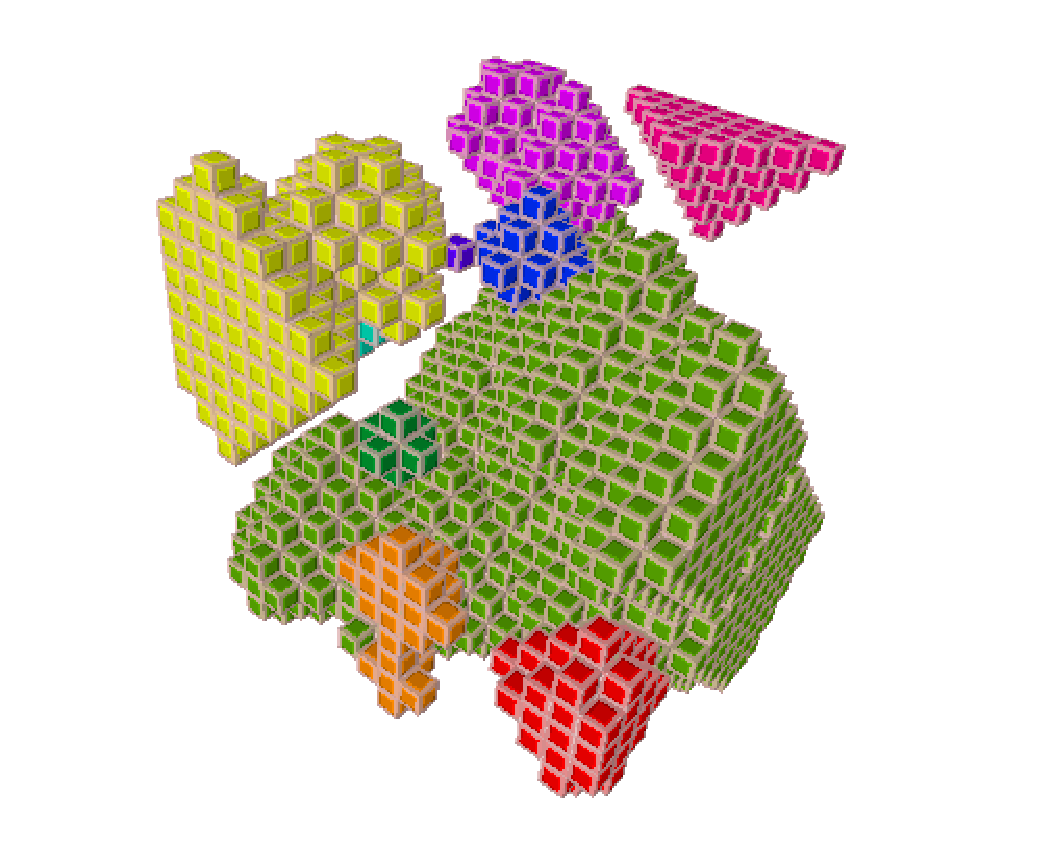
\includegraphics[height=0.22\textwidth]{Images/KSurfelsConnectedOrientExt.eps} &
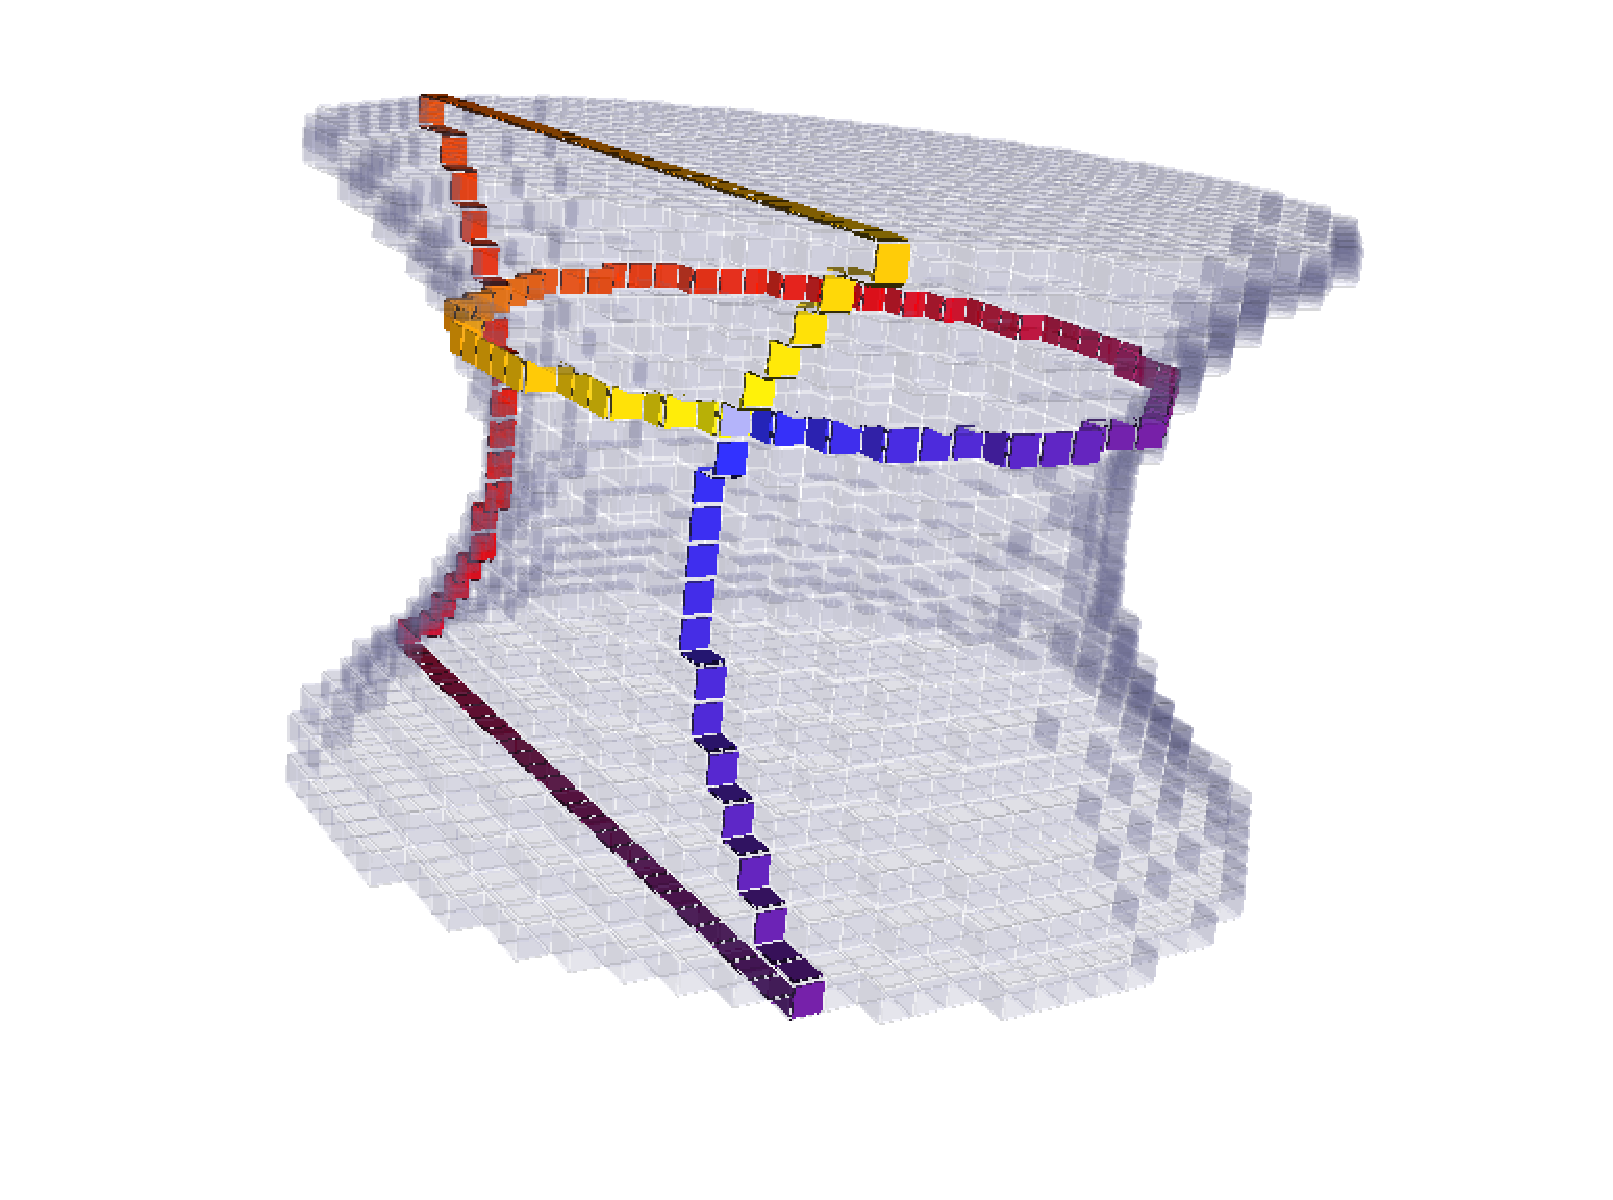
\includegraphics[height=0.22\textwidth]{Images/surfelTracking.eps}&
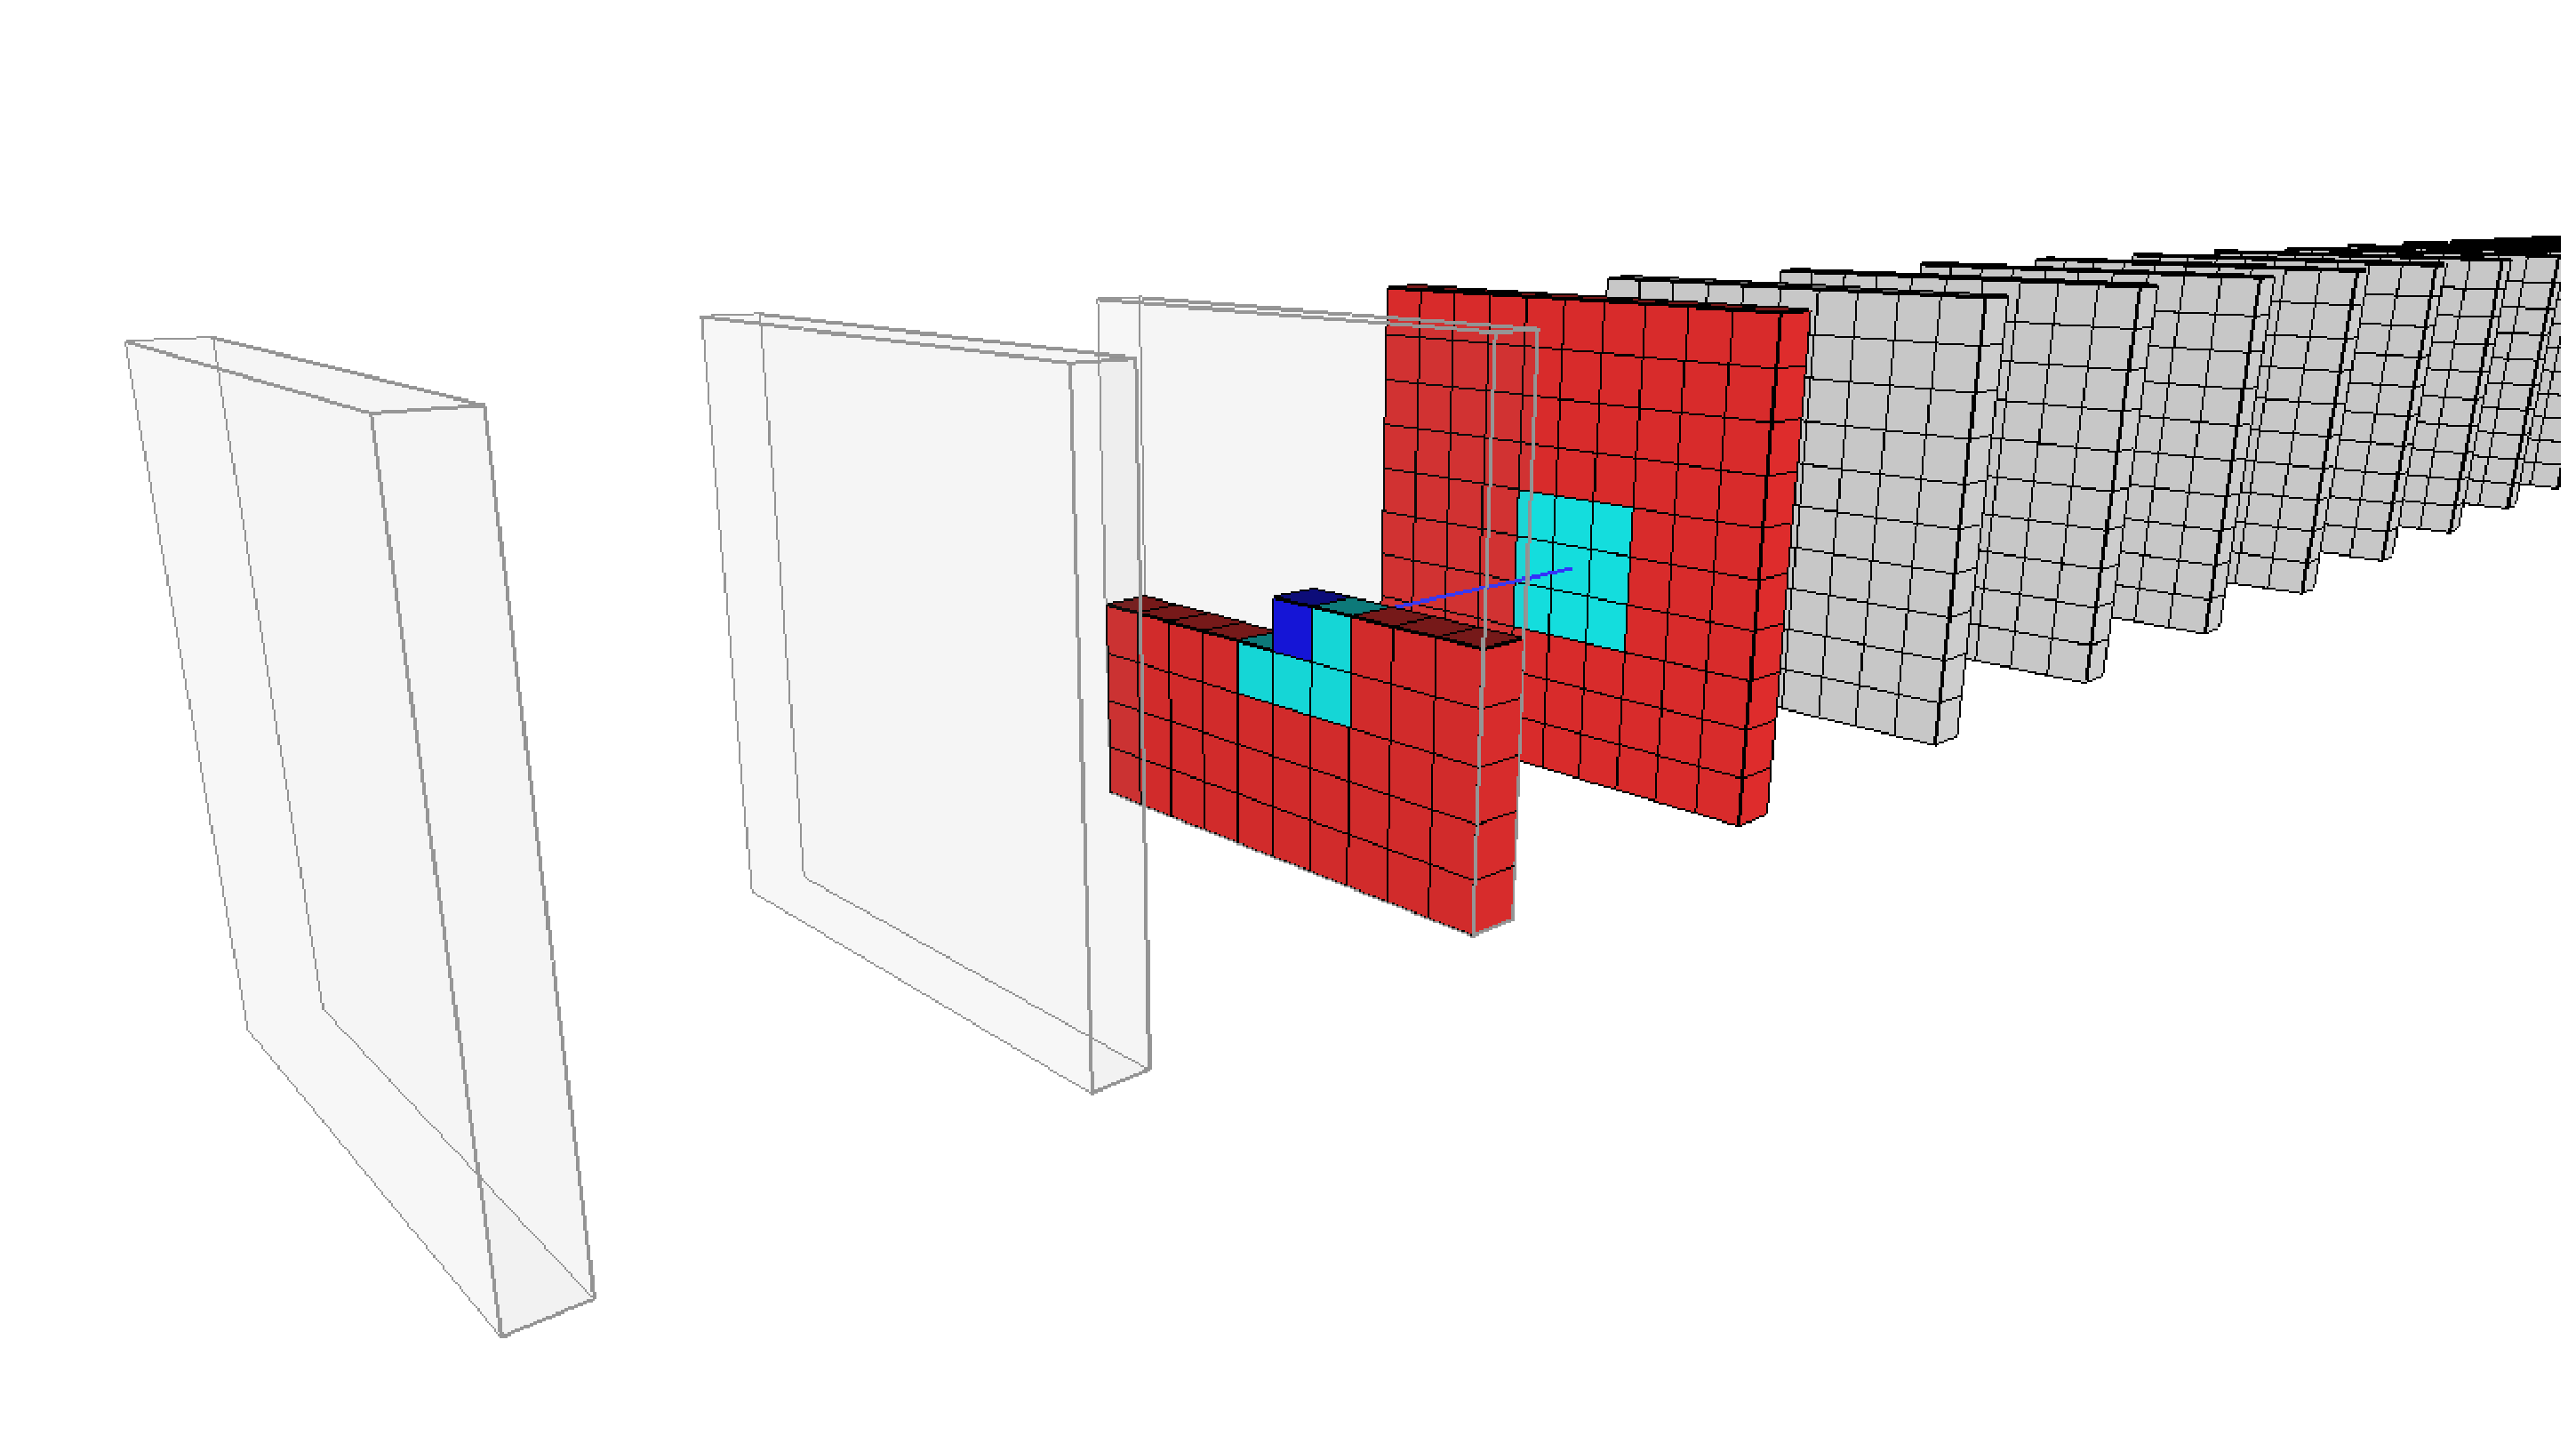
\includegraphics[height=0.2\textwidth]{Images/illustration3Dscan.eps} \\
{\scriptsize{Composantes connexes }}  & {\scriptsize{Suivi de surfels }} 

\end{tabular}
\end{center}


\end{frame}



\begin{frame}[t]
\frametitle{Autres fonctionnalit�s}

\begin{minipage}{0.65\textwidth}
\begin{block}{}
\begin{itemize}
\item Clipping planes: \\
\begin{semiverbatim}
 viewer  \texttt{< \hspace{-0.2cm}<} ClippingPlane(1,0,0,-4.9);
 viewer  \texttt{< \hspace{-0.2cm}<} ClippingPlane(0,1,0.3,-10); 
\end{semiverbatim}
\item<3-> Importation de donn�es simplifi�e (visu volumique en moins de 50 lignes)..
\item<4-> Gestion de la transparence.
\end{itemize}

\end{block}
\end{minipage}
\only<1>{\rput(2.2,0){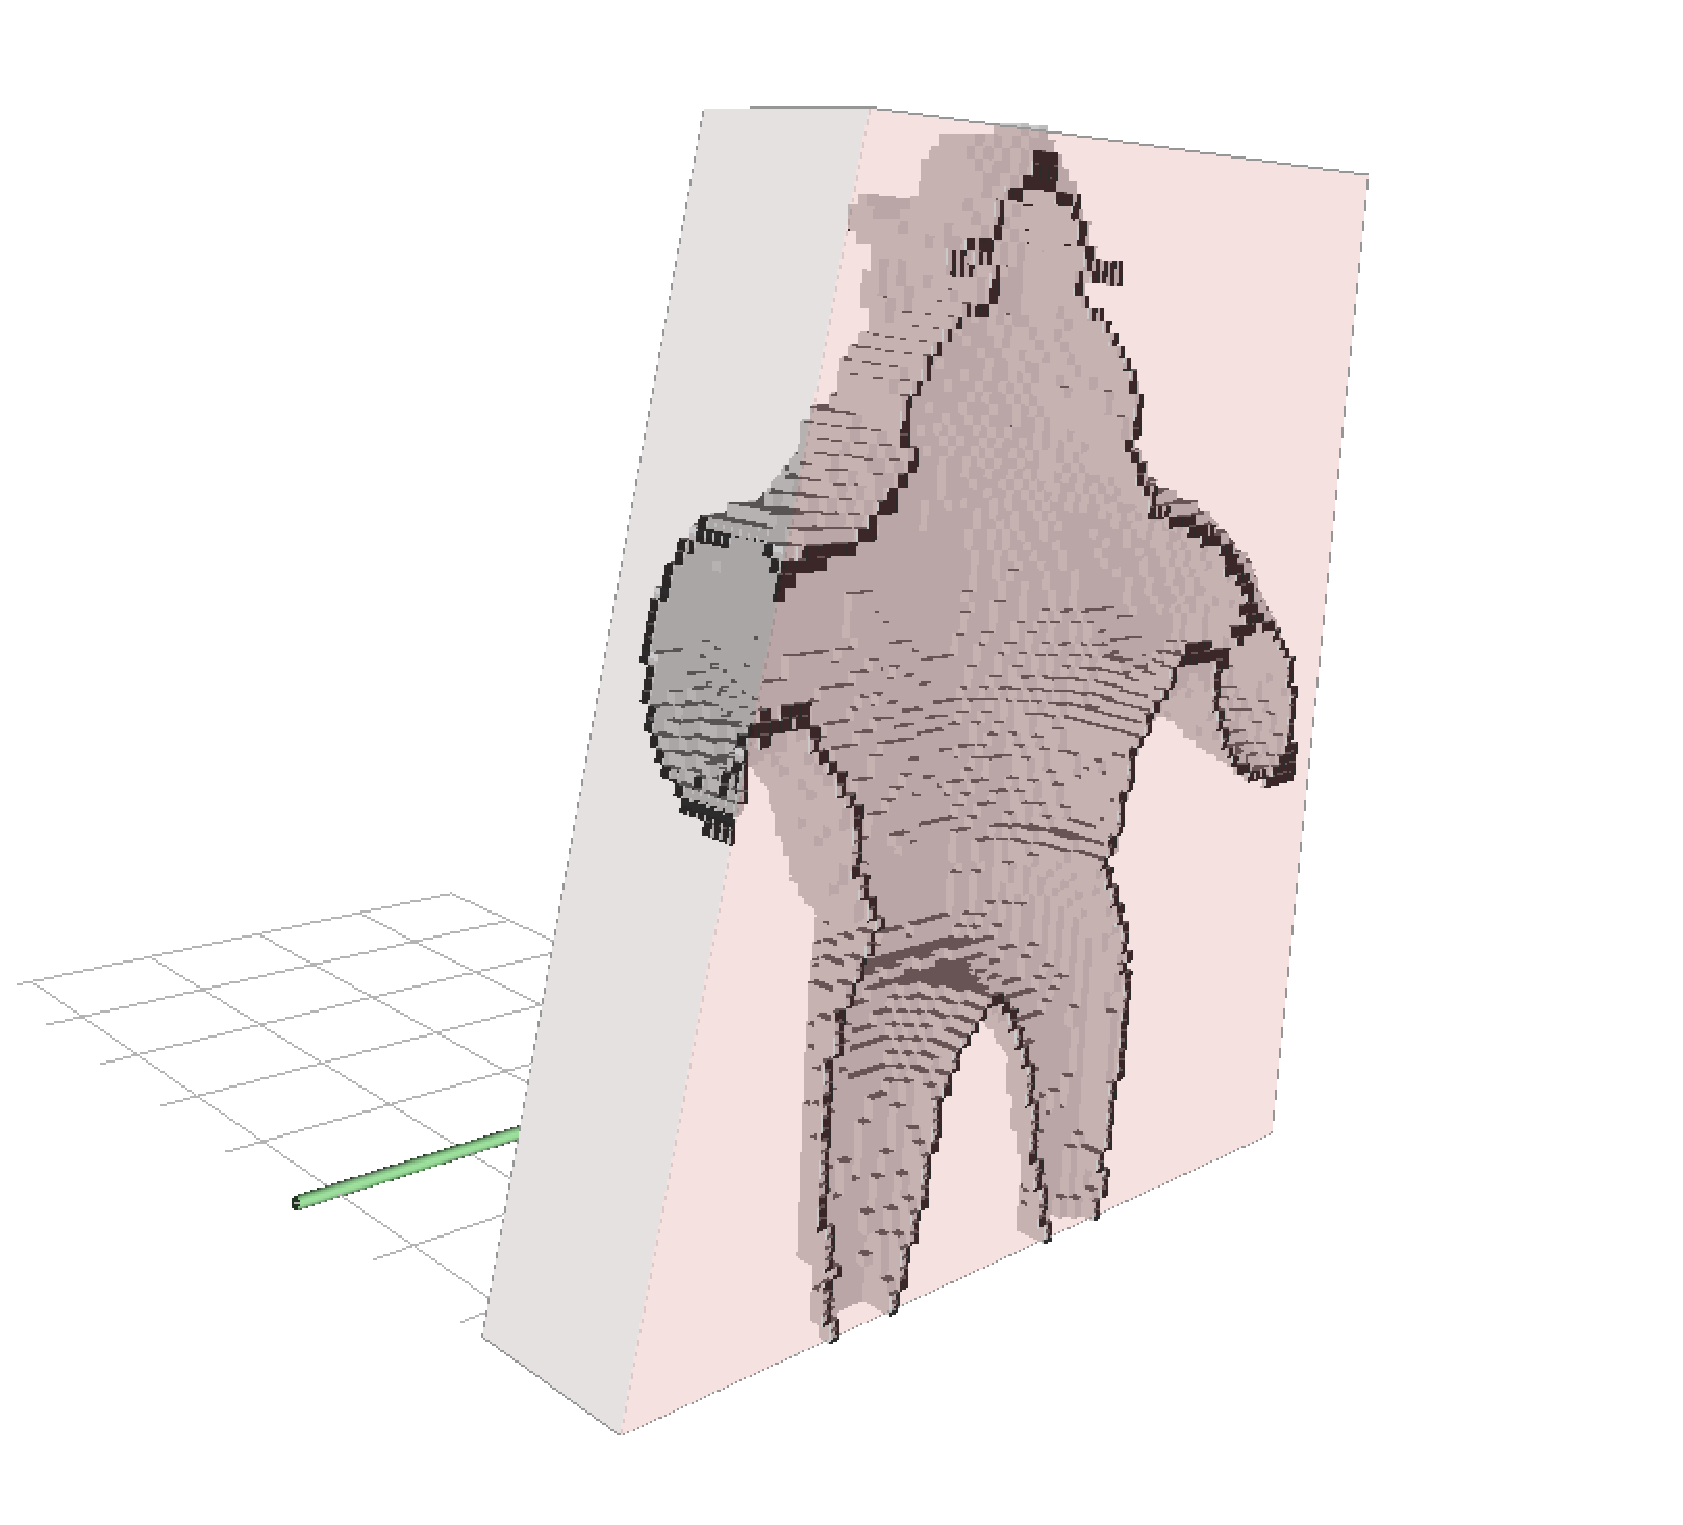
\includegraphics[width=0.3\textwidth]{Images/clipping1.eps}}}%
\only<2->{\rput(2.2,0){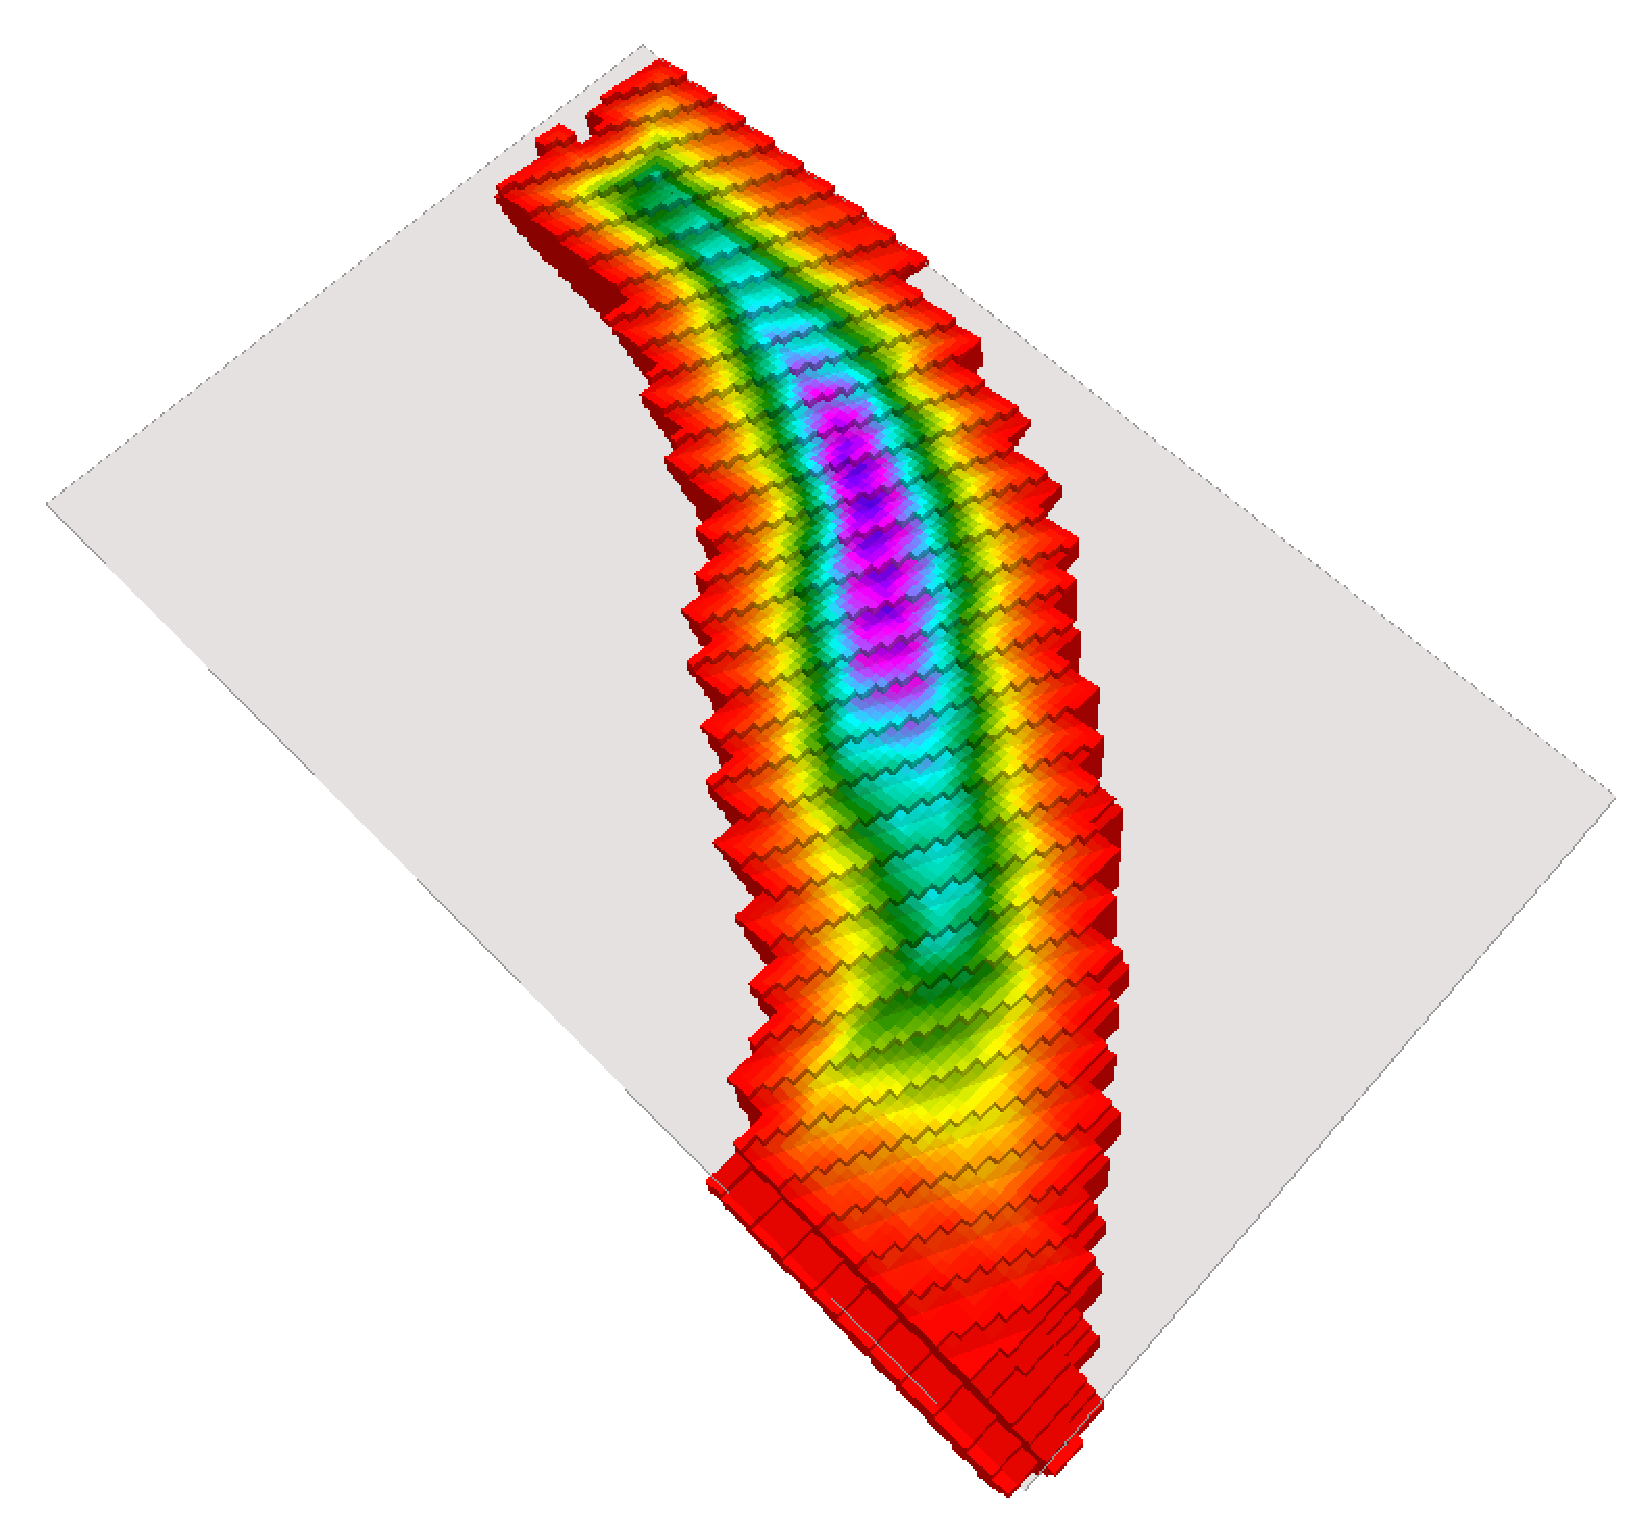
\includegraphics[width=0.3\textwidth]{Images/distanceMap.eps}}}%
\only<3>{\rput(-1.5,-3.6){\includegraphics[width=0.4\textwidth]{Images/visuVol3.eps}}}%
\only<4>{\rput(-1.5,-3.6){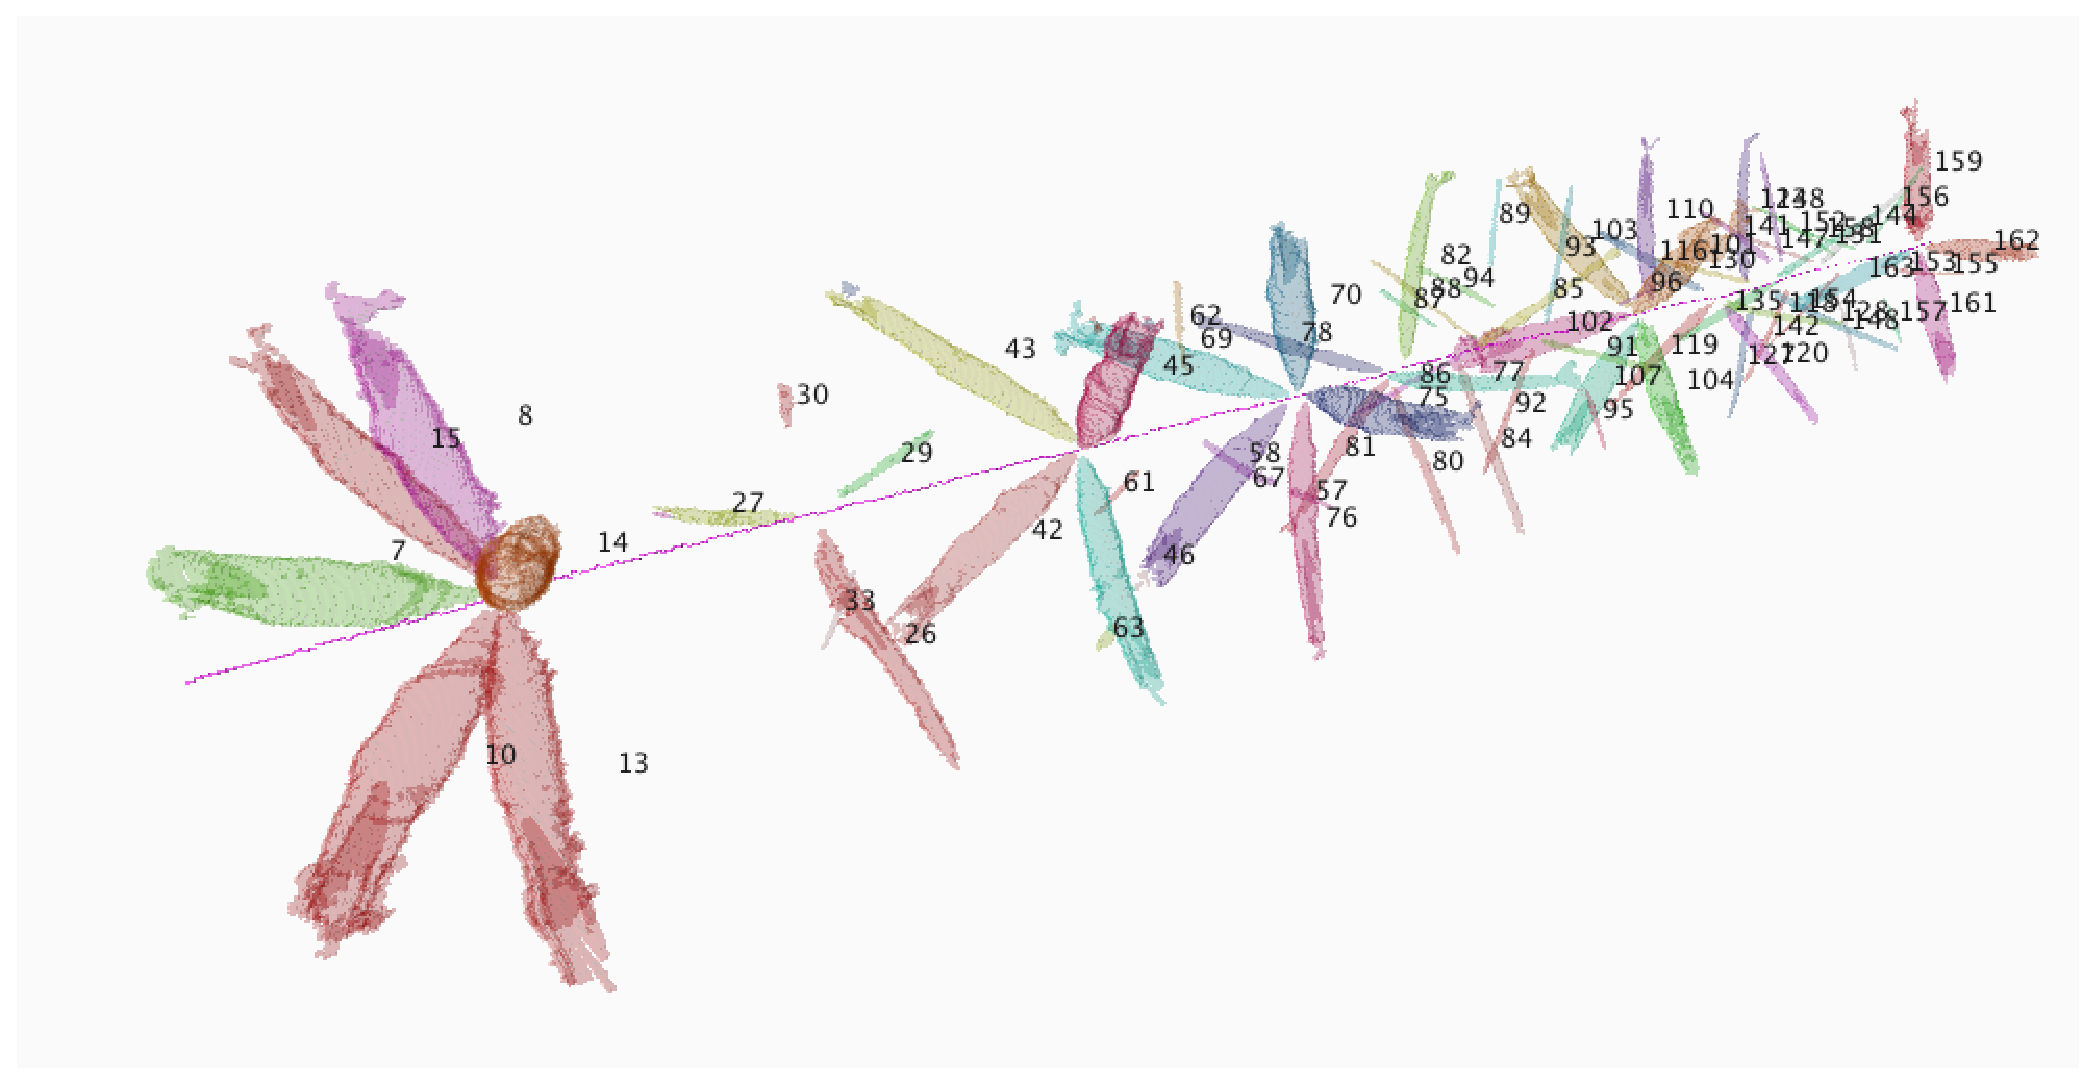
\includegraphics[width=0.6\textwidth]{Images/branche.eps}}}%

\end{frame}



\begin{frame}[c]
\frametitle{Exemple du code de l'outil de visualisation:}

\begin{center}
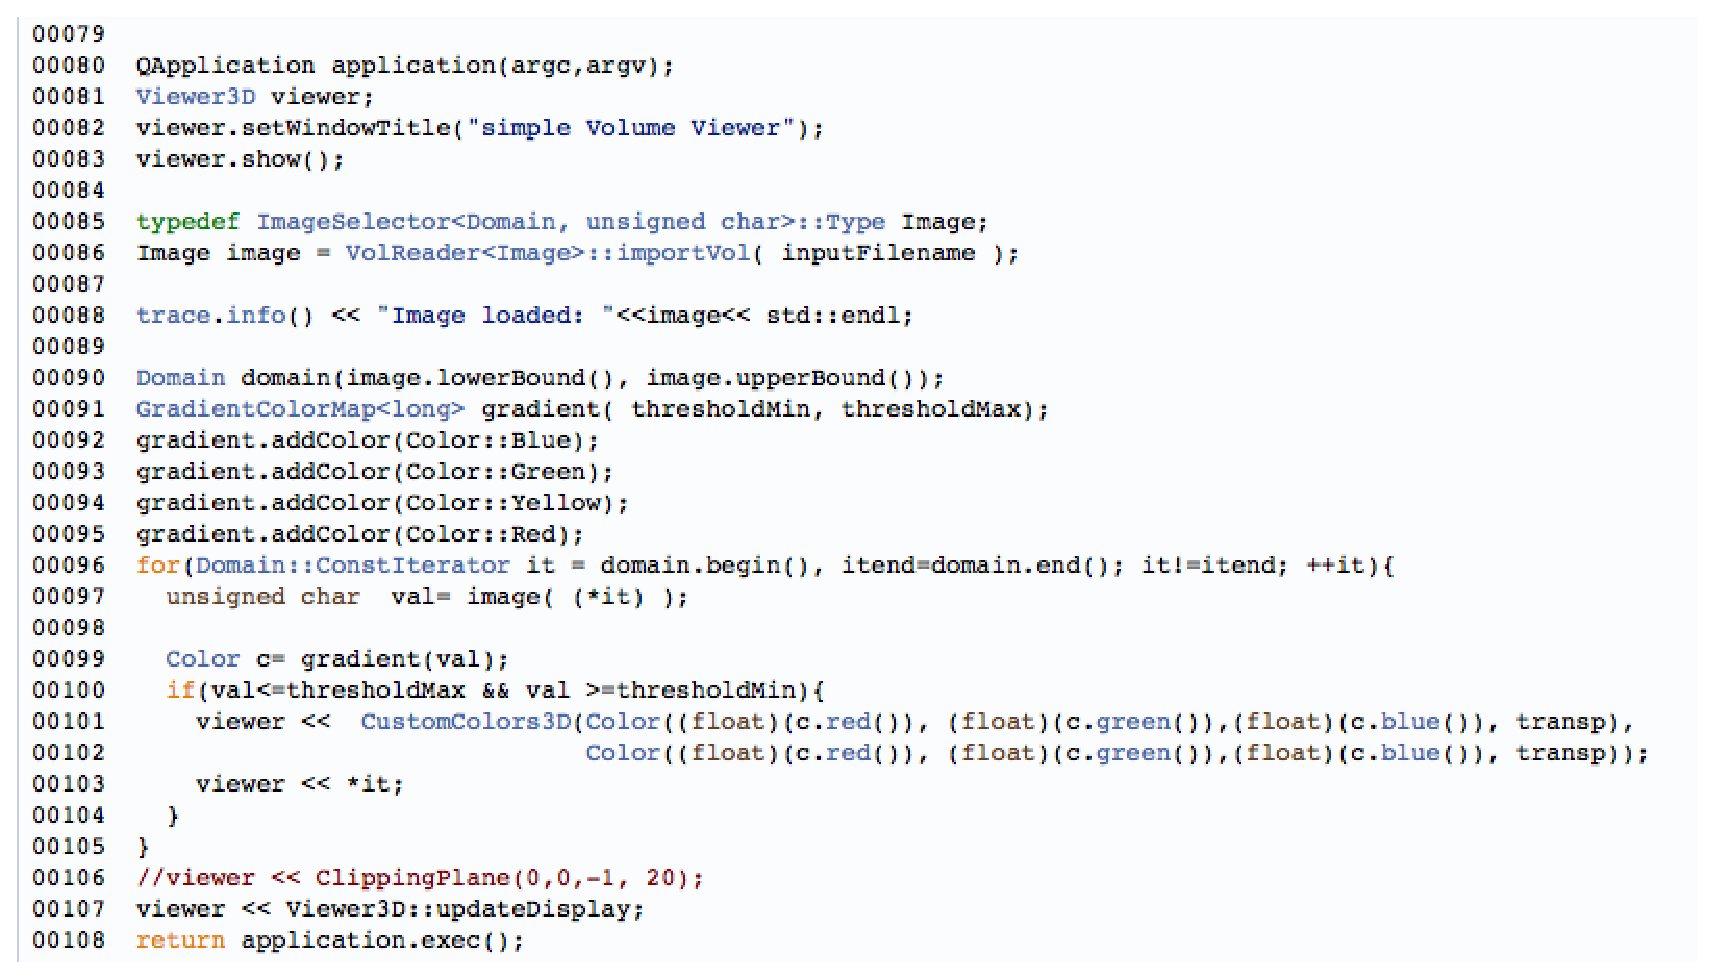
\includegraphics[width=0.9\textwidth]{Images/codeVisu3D.eps}
\end{center}


\end{frame}
